\documentclass[preprint]{aastex} %double-column, single-spaced document:
%\documentclass[iop,floatfix]{emulateapj} 

\usepackage[breaklinks,colorlinks,urlcolor=blue,citecolor=blue,linkcolor=blue]{hyperref}
\usepackage{graphicx}
\usepackage{apjfonts}
\usepackage{enumerate}
\usepackage{amsmath,amssymb}
\usepackage{bm}
\usepackage[usenames,dvipsnames,svgnames,table]{xcolor} 
\usepackage[utf8]{inputenc}

%version-control tagging based off of github.com/bd-j/speccal
%%% This file is generated by Makefile.
\newcommand{\githash}{a2871c4}\newcommand{\gitdate}{2014-08-19}\newcommand{\gitauthor}{Ian Czekala}

\newcommand{\prob}{{\rm prob}}
\newcommand{\qN}{\{q_i\}_{i=1}^N}
\newcommand{\qM}{\{q_{im}\}_{i=1,m=0}^{N,M}}
\newcommand{\yN}{\{y_i\}_{i=1}^N}

%\vt stands for ``vector theta''
\newcommand{\vt}{ {\bm \theta}}
\newcommand{\vg}{\vt_{\star, {\rm grid}}}
\newcommand{\vpp}{\vt_{\star, {\rm post}}}
\newcommand{\finst}{f_{\lambda, {\rm inst}}}
\newcommand{\fsynth}{f_{\lambda, {\rm synth}}}
\newcommand{\vN}{\vt_{\rm N}}
\newcommand{\vtstar}{\vt_{\star}}
\newcommand{\vtcheb}{\vt_{\rm Cheb}}
\newcommand{\vtglobal}{\vt_{\rm global}}
\newcommand{\vtorder}[1]{\vt_{{\rm order}_{#1}}}
\newcommand{\vtorders}{\vt_{\rm orders}}
\newcommand{\vtline}[1]{\vt_{{\rm line}_{#1}}}
\newcommand{\vtlines}{\vt_{\rm lines}}
\newcommand{\vtcov}{\vt_{\rm cov}}
\newcommand{\fM}{ \vec{{\bm M}}}
\newcommand{\fMi}{M_i}
\newcommand{\fD}{ \vec{{\bm D}}}
\newcommand{\fDi}{D_i}
\newcommand{\fR}{ {\bm R}}
\newcommand{\dd}{\,{\rm d}}
\newcommand{\trans}{\mathsf{T}}
\newcommand{\Z}{[{\rm Fe}/{\rm H}]}
\newcommand{\A}{[\alpha/{\rm Fe}]}
\newcommand{\matern}{Mat\'{e}rn}

\newcommand{\todo}[1]{ \textcolor{Blue}{\\TODO: #1}}
\newcommand{\comm}[1]{ \textcolor{Red}{SA: #1}}


%% Nomenclature guide
%%%%%%%%%%%%%%%%%%%%%
% * collections of synthetic spectra are generically called ``libraries.'' The term 
% ``grid'' is used when referring specifically to the spacing of spectral parameters
% in the library 

\shorttitle{Spectroscopic inference}
\shortauthors{Czekala et al.}

\begin{document}

\graphicspath{{figs/}}

\title{A Method for the spectroscopic inference of fundamental stellar parameters}
\author{\today{}\\
\medskip
Ian~Czekala\altaffilmark{1} et al.
%Author2\altaffilmark{2},
}

\altaffiltext{1}{Harvard-Smithsonian Center for Astrophysics, 60 Garden Street 
 MS 10, Cambridge, MA 02138}
%\altaffiltext{2}{Institution 2}
\email{iczekala@cfa.harvard.edu}

\section{Introduction}
\begin{itemize}
  \item Where our technique fits in the ecosystem of stellar methods.
  \item Applicable to any kind of spectrum (long-slit, echelle, infrared,
    flux-calibrated or not)
  \item Examples of fields where accurate and unbiased stellar parameters are
    crucial. Exoplanets. T Tauri stars.
\end{itemize}

\section{Method}

A single spectrum provides a wealth of information that can be used to infer the fundamental properties of a star: effective temperature $T_{\rm eff}$, surface gravity $\log g$, and metallicity $\Z$; together $\vg$. We wish to extract the maximal amount information from a given spectrum while also recognizing the limitations imposed by our stellar model and exposing any degeneracies between the parameters.  For example, if we model a large range of the spectrum at once (e.g., the full optical range at high resolution), then we must explicitly account for any covariances and biases introduced by improper calibration or inaccuracies in the model spectrum. We present a generative model which uses a synthetic stellar library as a backend and apply post-processing techniques to mimic the observed spectrum as a function of several stellar parameters and calibration parameters in order to determine the best fit. By forward modelling the data spectrum in a Bayesian framework, our modular approach can easily incorporate additional calibration artifacts and stellar complexity (e.g., veiling or Zeeman splitting) while still being true to the limitations of the dataset.  This data driven approach will enable us to learn how the underlying synthetic models may be improved and refined in an iterative manner.  

The roadmap for our method is as follows.
 First, for a given set of fundamental stellar parameters $\vg$, we generate a synthetic
 spectrum by interpolating from a grid of synthetic spectra (\S\ref{subsec:synthetic}). 
Then, we post-process the interpolated spectrum for realism by using additional
 parameters to describe Doppler shift, projected rotational velocity,
 interstellar extinction, and residual flux calibration errors
 (\S\ref{subsec:postprocess}). 
We perform a pixel-by-pixel comparison of the generated spectrum with the
 data spectrum using a prescribed likelihood function
 (\S\ref{subsec:likelihood}) and a parametric treatment of the covariance
 between pixel residuals (\S\ref{subsec:covariance}). 
We use a Markov chain Monte Carlo (MCMC) Gibbs sampler to numerically explore
the posterior probability density and determine constraints on the stellar
and nuisance parameters (\S\ref{subsec:MCMC}). 
The benefit of our method is that it provides robust estimates of the stellar and nuisance
parameters with well-quantified uncertainties and parameter degeneracies. 
Our parameterization of the covariance between pixel residuals also yields a means to identify
 and quantify the key discrepancies between the data and model, and provides a path forward to 
 improve the stellar models in an iterative fashion (\S\ref{subsec:learning}).
 \todo{I really want to overload the word ``covariance'' and use it to describe both the covariance between $T_{\rm eff}$ and $\log g$ as well as the covariance structure of the pixel residuals themselves. However I think this might be confusing so I am using ``degeneracies'' for the former and reserving ``covariance'' for the later.}

\subsection{Synthetic Model Spectra}
\label{subsec:synthetic}
Many methods exist to generate a synthetic model of a stellar spectrum. Generally, when
a high quality spectrum is needed for a specific set of stellar parameters, one
runs a stellar atmosphere and radiative transfer code to synthesize the
spectrum. Unfortunately, it is computationally expensive to accurately generate
a spectrum over a wide range of wavelengths, and so these codes are generally
employed to generate libraries of stellar spectra, which exist over a range of
$\vg$ at specified points on a regular grid, typically covering the main sequence of stellar
types. Several high-quality libraries of synthetic spectra now exist
(\citealt{hwd+13}, Kurucz, and more are being developed for GAIA).  

In a forward-modelling approach, which may make many calls to generate a
spectra of varying $\vg$, it is currently computationally impractical to
iterate the structure of the stellar atmosphere and then run the stellar
synthesis for each call of $\vg$.  Some methods compromise by taking a halfway
approach, whereby a precomputed library of stellar atmospheres is interpolated
for a given $\vg$, and then a simple radiative transfer code is run to
synthesize a spectrum (e.g.  SME; \citealt{vp96}). This technique has the
advantage that interpolating atmospheres and then running the spectral
synthesis for each $\vg$ might be more accurate than directly interpolating
synthetic spectra. However, if a large region of wavelength is required at high
resolution, then the synthesis step will be slow.  A different approach might
be instead to eschew forward modelling (and thus repeated synthesis or grid
interpolation) of the spectra entirely and evaluate the posterior probability
density only at the grid points of the spectral library.  Then, these discrete
samples of the posterior density can be interpolated to find the posterior
surface and draw confidence intervals on the parameters (e.g. SPC;
\citealt{blj+12}). However, the difficulty with this approach is that the
parameter uncertainty might be smaller than the grid spacing, and then
interpolation will not properly capture degeneracies between parameters.

Because we desire a generative model of the spectra without the added
complexity or computational overhead of running a stellar synthesis, we opt to
use a \todo{Implement a more accurate but still fast interpolator for the grid.
Likely this will be a combination of using splines to pre-interpolate a finer
grid (~20 K, 0.1 dex spacing in gravity and metallicity and then doing linear
interpolation off of this new grid during the actual MCMC run. It will be described here.} However, the
techniques we develop in this paper to account for and parameterize the
correlated, systematic pixel residuals are generally applicable to spectra fit
by any of these methods.


\begin{figure*}[!htb]
\begin{center}
  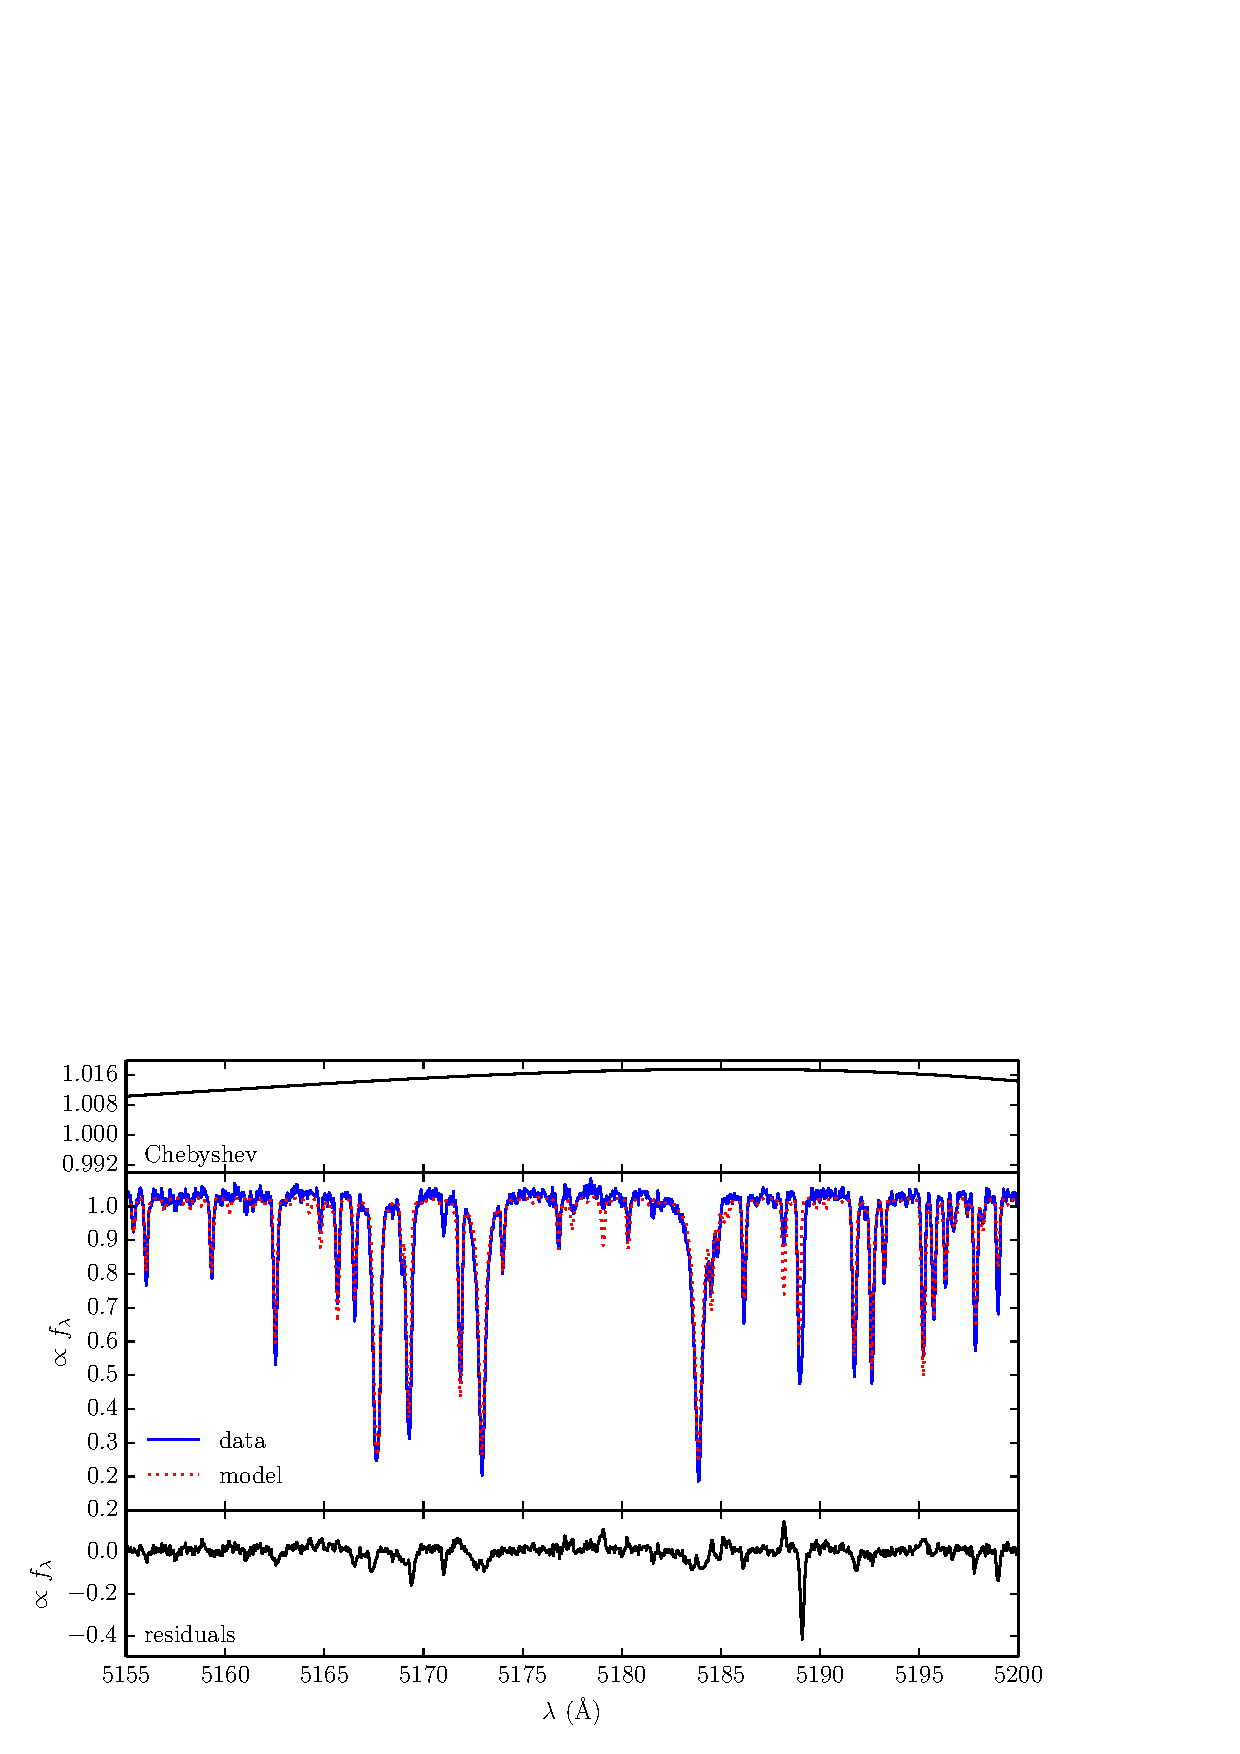
\includegraphics[width=0.85\textwidth]{figs/model_data.pdf}
  \caption{\textbf{Top}: Chebyshev polynomial which multiplies the model spectrum
   to account for inaccuracies in the flux-calibration. 
  \textbf{Middle}: The data spectrum and model spectrum, after it has been
   interpolated, post-processed, and multiplied by the Chebyshev polynomial.
  \textbf{Bottom}: Residuals from the model fit. Note the large residual at
   $\lambda5189$\AA\ due to a missing opacity source from \ion{Ca}{2}.}
\label{fig:model_data}
\end{center}
\end{figure*}


\subsection{Post-Processing}
\label{subsec:postprocess}

Libraries of synthetic spectra are generally computed at high resolution ($R
 \geq $100,000), sampled with many pixels per resolution element, and do not
 include any rotational broadening or account for any instrumental effects. 
In order to transform a raw synthetic spectrum interpolated from the grid into
 one that matches the spectrum of a real star, we must post-process the spectrum
 to account for these secondary effects. 
In addition to these fundamental parameters, a star also has several observed
 properties that are a function of its kinematics, geometry, and location in our
 galaxy: projected rotational velocity $v \sin i$, line of sight velocity $v_z$,
 total extinction $A_V$, and solid angle $\Omega$. 
We call these secondary parameters $\vpp$, because we can model their effects
 on the synthetic spectra in a ``post-processing'' step by convolution with an
 appropriate kernel or multiplication with a smooth function. 
Together, we call $\vtstar = \{\vg, \vpp\}$.

The projected rotational velocity of the star, parameterized by $v \sin i$,
broadens spectral line profiles and is mathematically described by convolution
with a specific kernel \citep[Equation 18.14]{gra08}. UV, optical, and infrared
spectra are acquired using a spectrograph which disperses light onto a CCD,
defining a specific resolution and sampling rate for the spectrum.  Because the
resolution of the spectrograph and pixel sampling are different from the
synthetic spectral library, we must convolve the raw spectrum with the line
spread function (LSF) of the instrument and resample to the exact pixels of the
CCD. In wavelength space, the $v \sin i$ and LSF operations are represented by
the convolution of the synthetic spectrum with these two kernels.  Using the
convolution theorem, we can rewrite these convolutions as multiplications in
Fourier space.  In order to use the fast Fourier transform (FFT) with discrete
samples of the synthetic spectrum, we must first resample it
onto a uniform grid.  In the case of a spectrum, the natural
uniform grid is one that is equally sampled in velocity space, such there is an
equal velocity shift $\Delta v$ between pixels. This results in a wavelength
grid that is linearly sampled in the logarithm of wavelength.  Next, we
multiply the Fourier transform of the synthetic spectrum by the Fourier
transforms of the rotational velocity and line spread function kernels.
Lastly, we do an inverse FFT to transform the modified spectrum back to
wavelength space, where it is sampled at the wavelength locations of the pixels
in the detector.  When resampling the spectrum, we are careful to ensure
band-limited interpolation using splines in order to prevent introducing
non-physical high frequency structure into the spectrum.  

We scale the raw synthetic flux (often reported at the stellar surface) to an
observed flux by multiplying by the solid angle of the star, $\Omega =
R_\star^2/d^2$, where $R_\star$ is the stellar radius and $d$ is the distance
to the star from earth. Then, we correct for a radial velocity difference $v_z$ between the
star and the earth by Doppler shifting the model spectrum.  Finally, we correct
for interstellar extinction by dividing by a dust extinction model
$A_\lambda$, which is parameterized by extinction in the $V$ photometric band,
$A_V$. 
\todo{We can add in convolution with photometric filter
profiles to use photometry and provide a better constraint on the luminosity of
the star}
\todo{We might try implementing the convolution in wavelength space, rather
 than the FFT. 
This would allow the LSF to change with wavelength.\\} 


\paragraph{Calibration polynomials} In contrast to a collection of photometric points in a spectral energy distribution, or any ensemble of data for which each data point is acquired by an individual measurement, adjacent wavelength points in a spectrum are measured simultaneously, with the same detector and--more importantly--the same calibration. Typically, spectra are flux calibrated by dividing by a ``sensitivity function,'' which is determined by comparing an observation of a spectrophotometric standard to a previously calibrated model spectrum. Therefore, any error in the sensitivity function, which is typically a smooth function with wavelength, will create a region of the data spectrum which is systematically offset by a small amount from what the true flux should be. The flux calibration error is then the residual difference in the empirically determined sensitivity function from the what the ``true'' sensitivity function would be if we had a perfectly calibrated instrument and spectrophotometric standard. Therefore, it is necessary to introduce additional degrees of freedom into our model in order to account for the calibration error and allow the model spectrum to properly match the data. By adding the residual calibration as a parameter in our model, we can explore the distribution of possible calibrations (\S\ref{subsec:MCMC}) and then marginalize the calibration parameters out of the final posterior distribution of the stellar parameters. This means that we can derive estimates of stellar parameters that properly account for the intrinsic uncertainty in the flux calibration.

A traditional way to deal with errors in the flux calibration is to avoid flux-calibration entirely and simply normalize both the data and the spectrum to the continuum level before comparison.  While this procedure may work well for hotter stars with well-defined continuua, normalizing spectra of cooler stars with large molecular features may introduce artificial features into the spectrum when the pseudo-continuum is incorrectly placed.  Instead, we choose to parameterize the residual flux calibration error by a low-order Chebyshev polynomial which is normalized to unity. The coefficients of the polynomial are parameters in the model that will be determined by the fitting algorithm, $\vtcheb = \{c_0, c_1, \ldots, c_N \}$. If we have multiple observations of spectrophotometric standards, then we can characterize the typical flux-calibration error of the spectrograph and put priors on the coefficients that will prevent overfitting of the polynomials.  For an example of the Chebyshev polynomial determined for a typical spectrum, see Figure~\ref{fig:model_data}. Using priors on the Chebyshev coefficients ensures that real spectral features, such as deep molecular bands in later type stars, are not accidentally treated as calibration artifacts. The overall normalization of the polynomial $c_0$ is degenerate with the solid angle of the star $\Omega$. Therefore we apply an additional constraint and enforce that the mean of the Chebyshev polynomial be equal to $1$. If there is only one order in the spectrum, such as with a long-slit spectrum or a single order of an echelle spectrum, then this means setting $c_0 = 1$. If we are fitting more than one order of an echelle spectrum then we adopt an independent Chebyshev polynomial for each order. This means that we chose the $c_0$ of a specific order to anchor to 1, while the $c_0$ for other orders are allowed to take on perturbations about $1$. 

This polynomial formalism can in principle be used to model raw (not flux calibrated) spectra by using the Chebyshev polynomial to solve directly for the sensitivity function itself, rather than a residual calibration error as is currently done. When used in this manner, there will be greater uncertainty about the properties of the spectrograph, which will translate into wider priors on the Chebyshev coefficients.  In this case, there is more of a chance that the polynomial might destroy broad-scale information present in the spectrum by fitting it out, something that would be avoided with more accurate priors provided by a flux calibration.

\subsection{Likelihood Calculation}
\label{subsec:likelihood}

To evaluate which parameters of the model spectrum fit the data spectrum best,
we use a likelihood function to compare individual pixels between the two
spectra. A likelihood function provides the probability of the data spectrum
$\fD$, given the model spectrum $\fM(\vt)$, which is parameterized by the
stellar and calibration parameters $\vt$. The data spectrum and model spectrum are both composed of $N$ pixels, and so $\fD$ and $\fM$ represent the collection of these pixels in vector form, 
$\fD = \{\fDi\}^N_{i=1}$ and $\fM = \{\fMi\}^N_{i=1} $, respectively. The vector of residuals is the difference between the data spectrum and the model spectrum
\begin{equation}
  \fR(\vt) = \fD - \fM(\vt)
\end{equation}
In the language of probability calculus, the likelihood function is written as
$p(\fD | \fM(\vt))$, or $p(\fD | \vt)$ for short. We choose a standard
multidimensional Gaussian likelihood function which allows for covariance
between the pixel residuals 
\begin{equation}
  p(\fD | \vt) = \frac{1}{\sqrt{(2 \pi)^N \det(C)}} \exp\left ( -\frac{1}{2}
   \fR^T C^{-1} \fR \right ) 
   \label{eqn:prob}
\end{equation}
which penalizes models that yield larger residuals. $C$ is the covariance
matrix which describes the covariance between the pixel residuals. The structure of the covariance matrix is discussed in detail in the next section (\S\ref{subsec:covariance}). Because
the likelihood function generally exhibits a large dynamic range, it is numerically
preferred to use the log-likelihood function
\begin{equation}
  \ln[p(\fD | \vt)] = -\frac{1}{2} \fR^T C^{-1} \fR - \frac{1}{2} \ln \det C  
   - \frac{N}{2} \ln 2 \pi 
  \label{eqn:lnprob}
\end{equation}


\subsection{Parameterizing the covariance structure}
\label{subsec:covariance}
The covariance matrix $C$ describes the measurement noise in each pixel of the spectrum as well as the covariance between pixel residuals. It is fundamental to the likelihood calculation described in \S\ref{subsec:likelihood}. For most problems, such as fitting a spectral energy distribution to photometric measurements, each data point is acquired in an independent measurement from the other data points, which means that the noise for each data point, $\sigma_i$, is also independent from the other data points. This results in a diagonal covariance matrix
\begin{equation}
  C = 
  \begin{bmatrix}
    \sigma_0^2 & 0  & \cdots & 0\\
    0 & \sigma_1^2 & \cdots & 0\\
    \vdots  &   & \ddots  & \vdots \\
    0 & 0 & \cdots & \sigma_N^2\\
  \end{bmatrix}
  \label{eqn:covariance_diagonal}
\end{equation}
with $\sigma_{ij} = \delta_{ij} \sigma_{ij}$, where $\delta_{ij}$ is the Kronecker delta function. When the covariance matrix is diagonal, 
the likelihood function (Equation~\ref{eqn:lnprob}) reduces to the familiar
$\chi^2$ form of a sum over the square of the residuals, weighted by the
inverse variance of each data point
\begin{equation}
  \ln[p(\fD | \vt)] \propto - \frac{1}{2} \chi^2 = - \frac{1}{2} \sum_i^N
   \frac{R_i^2}{\sigma_i^2}
   \label{eqn:chi2}
\end{equation}

\begin{figure*}[!htb]
\begin{center}
  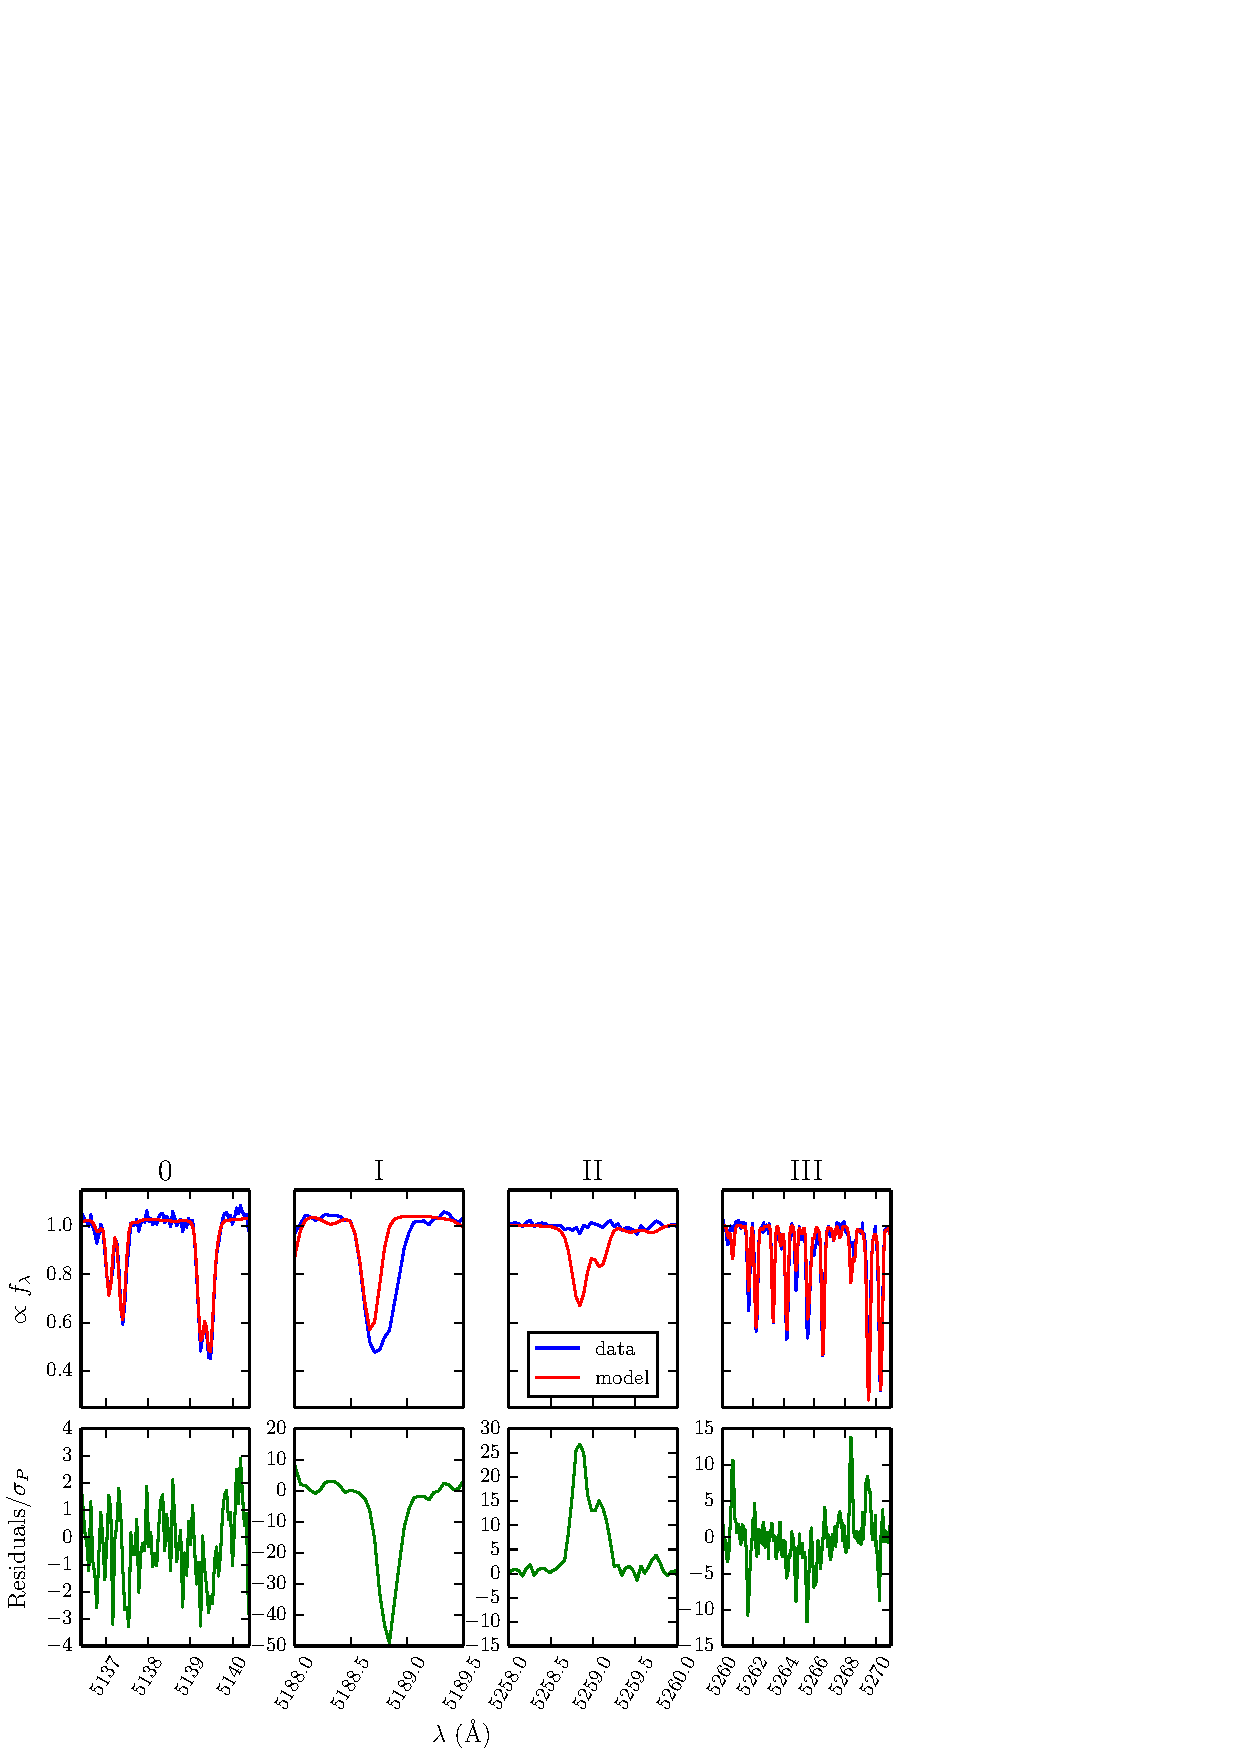
\includegraphics{figs/badlines.pdf}
  \caption{A collection of spectral lines which have imperfect model fits.
    From left to right: \textbf{Class 0} The majority of spectral lines
    ($\gtrsim 60$\%) will have minor differences in strength between data and
    model spectrum, which produce low-amplitude correlations in the residuals
    on the length scale of the width of a typical spectral line.  \textbf{Class
    I}: Sometimes ($\lesssim 5$\% of all lines), a missing opacity source in
    the model (in this case a line-blended \ion{Ca}{2}) leaves a large, highly correlated
    patch of negative residuals.  \textbf{Class II}: Sometimes ($\lesssim 5$\%
    of all lines), an extraneous line in the model leaves a large, highly
    correlated patch of positive residuals.  \textbf{Class III}: If the line strengths are
    substantially discrepant ($\lesssim 10$\% of all lines), there will be many
    correlated residuals of moderate amplitude.  The difficulty
    with class III lines is that for any specific line, there might exist a
    $\vtstar$ that will fit the line, but there does not exist a $\vtstar$ that
    will properly fit \emph{all} the lines.}
\label{fig:badlines}
\end{center}
\end{figure*}

However, the pixel residuals from a spectroscopic fit will often be correlated and will invalidate Equation~\ref{eqn:chi2}. These correlations arise because the CCD pixels of a spectrograph do not sample independent wavelengths of the spectrum. Instead, spectrographs are designed so that the LSF is properly sampled by at least a few pixels, meaning that adjacent pixels do not sample completely independent parts of the spectrum. Because of this, when a spectral feature differs between the model and the data, it creates a residual which spans several adjacent data points. For a collection of correlated residuals produced by a typical spectroscopic fit, see Figure~\ref{fig:badlines}. 

\begin{figure*}[!htb]
\begin{center}
  $\vcenter{\hbox{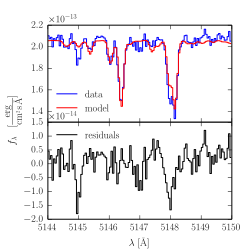
\includegraphics{figs/class0_residuals.pdf}}}$
  $\vcenter{\hbox{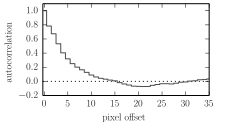
\includegraphics{figs/class0_autocorrelation.pdf}}}$
  \caption{\textbf{Left} The same residuals from Figure~\ref{fig:badlines}, panel 0, but enlarged to show the mildly covariant structure produced by slight mismatch between the data and model spectra.   
  \textbf{Right} The autocorrelation (Equation~\ref{eqn:autocorrelation}) of the residual sequence shown at left. Notice that there is significant correlation for offsets of $\lesssim 4$ pixels.}
\label{fig:class0}
\end{center}
\end{figure*}

There is an important distinction between astrophysical or instrumental ``noise'' and the residuals from a spectroscopic fit. Noise introduced to a spectrum by astrophysical or instrumental effects is generally uncorrelated with wavelength. This is because the arrival of each photon to the detector is a discrete event, and while photons are scattered by the LSF, the particular scattering direction of each photon is independent from any other photon. We can verify this by measuring the autocorrelation of residuals in a region of well-fit stellar continuum, and show that it is flat. If the model spectrum is \emph{perfect}, then the residuals from a spectroscopic fit will be uncorrelated and equivalent to the astrophysical and instrumental noise introduced into the measurement. However, when we compare a data spectrum and a model spectrum that have many absorption lines, even small differences will produce correlated \emph{residuals}. We can verify this correlation by estimating the autocorrelation of the residuals as a function of pixel offset $k$
\begin{equation}
  \hat{\rho}\,(k) = \frac{1}{(n - k)\,\sigma^2} \sum_{i = 1}^{n - k} (R_i - \mu_R)\,(R_{i+k} - \mu_R)
  \label{eqn:autocorrelation}
\end{equation}
over a region of spectrum of length $n$ pixels. Figure~\ref{fig:class0} shows a general residual structure induced by slight model mismatch and the autocorrelation of this series. There is significant correlation for offsets of $\lesssim 4$ pixels, which is also the typical width of a spectral line for this spectrum.

Although the correlation in the residuals is artificially induced by an
imperfect model fit rather than originating from a physical source of
correlated noise, we can treat these two effects as mathematically similar. By
using a non-trivial covariance matrix with off-diagonal terms we can describe
the small-scale covariance between pixel residuals shown in
Figures~\ref{fig:badlines}~and~\ref{fig:class0}. A non-diagonal covariance also
requires that we use  a likelihood function  which uses a matrix product instead of a sum over independent pixels (Equation~\ref{eqn:lnprob}).

We seek to understand and parameterize the structure of covariance in the
spectroscopic residuals, because ignoring this complexity will bias the estimates of
the model parameters $\vt$. As a simple analogy, consider the fit of a straight
line to a dataset.  If the noise in the dataset is correlated, then nearby
data points might be offset from the linear trend in the same direction by a
similar amount.  If the covariant structure of the noise is ignored, a simple
$\chi^2$ will treat these correlated offsets as due to the linear trend, which
will result in a biased determination of the slope and intercept of the line,
typically with uncertainties that are too small. We face a mathematically similar problem with 
correlated pixel residuals from a spectroscopic fit.

We parameterize the covariance structure using covariance kernels, taken from
the field of Gaussian processes. Covariance kernels describe the covariance
between two pixels $\lambda_i$ and $\lambda_j$.  These kernels are analogous to
the cosmological two-point correlation function, where the distance
between two galaxies is used instead of the wavelength of light.

\paragraph{Global and mildly covariant structure}
To account for the mild covariance structure shown in Figure~\ref{fig:class0},
which is generally low amplitude and has a correlation length of only a few
pixels but is present throughout the majority of the spectrum, we use a
\emph{stationary} covariance kernel. Stationary covariance kernels, also called \emph{radial basis functions}, satisfy the property that the
amount of correlation only depends on the distance between the two pixels $r$.  For spectra,
we map $r$ to the velocity difference between two pixels
\begin{equation}
  r\,(\lambda_i, \lambda_j) = \Delta v = \frac{c}{2} \left | \frac{\lambda_i 
   - \lambda_j}{ \lambda_i + \lambda_j} \right |
\end{equation}
Then the covariance kernel describes the expected covariance between pixel residuals
\begin{equation}
  k(\lambda_i, \lambda_j) =  \langle R_i \; R_j \rangle
  \label{eqn:expectation}
\end{equation}
In theory, we could chose from a plethora of covariance kernels to parameterize this mildly covariant structure, as long as they satisfy the property that the degree of covariance smoothly declines with increasing radial distance. In practice, there are a few covariance kernels which are well-respected within the machine-learning community and frequently employed to parameterize covariance of this nature \citep{rw05}. We choose to use the \matern\ $\nu = 3/2$ kernel because it is one of the most commonly used kernels for this purpose and has an extensive history of use (cite?). 
\begin{equation}
  k_{\nu = 3/2}(r\, |\, a_{\rm g},\, l) = a_{\rm g} \left(1 + \frac{\sqrt{3} r}{l} \right ) \exp 
   \left (- \frac{\sqrt{3} r}{l} \right )
\end{equation}
This kernel is an exponential tapered by a polynomial, which makes for a smooth transition from small scale covariance to negligible covariance at longer scales. In order to ensure sparsity of the covariance matrix for computational efficiency, we
 taper the \matern\ kernel for compact support using a Hann window
\begin{equation}
  w\,(r |\, r_0) = \left \{ 
    \begin{array}{cc}
    0.5 + 0.5 \cos (\pi r/ r_0 ) & r \le r_0 \\
    0 & r > r_0\\
  \end{array}
  \right .
  \label{eqn:Hann}
\end{equation}
for which we generally fix $r_0$ to be some fixed multiple of the length scale, say $r_0 = 4 l$. Then, if we define the global parameters $\vtglobal = \{a_g, l \}$, we have a final covariance kernel of 
\begin{equation}
  k_{\rm global} (r\,|\,\vtglobal) = w(r |\, r_0 = 4l)\; k_{\nu = 3/2}(r |\, a_{\rm g},\, l) 
  \label{eqn:global}
\end{equation}
\todo{This might be a good place to actually include a simple plot of $k_{\rm global}$ as a function of $r$, as long as we aren't providing too many figures. Maybe it could be combined with Figure~\ref{fig:matern}.}

We add this covariance kernel to the independent pixel noise $\delta_{ij} \sigma_{ij}$ already present along
 the matrix diagonal, and introduce an additional parameter to allow a constant rescaling of the independent noise. Then, each element of the covariance matrix is completely described by
\begin{equation}
  k(\lambda_i, \lambda_j |\vtglobal, \, b) = k_{\rm global}(r | \vtglobal) + b\,\delta_{ij} \sigma_{ij}
\end{equation}
Therefore, the \emph{hyperparameters} of this covariance kernel directly determine the structure of the covariance matrix. By varying the hyperparameters, we can create a covariance matrix which accurately mimics the correlated structure of the pixel residuals. Most importantly, when the hyperparameters are correctly chosen to properly model this correlated structure, the likelihood function will be maximized (Equation~\ref{eqn:prob}) while also encapsulating the true uncertainty in the spectroscopic fit.
 
\begin{figure*}[!htb]
\begin{center}
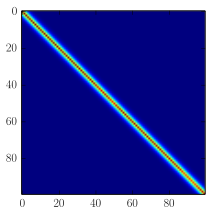
\includegraphics[width=0.4\textwidth]{figs/matern_matrix.pdf}
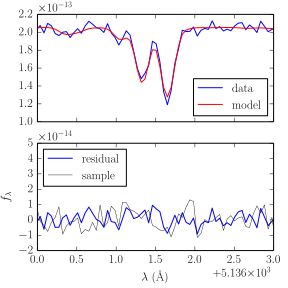
\includegraphics[width=0.4\textwidth]{figs/matern_draw.pdf}
\caption{\textbf{Left} Inset zoomed to show a small region of a typical covariance matrix, generated using the kernel in Equation~\ref{eqn:global} and common values for the hyperparameters. There is a small degree of covariance in elements within a few pixels off the diagonal, which quickly tapers off so that the majority of the matrix remains sparse ($\sigma_{ij} = 0$). This matrix is used to model a spectrum which is correlated on a $\sim$few pixel scale.
\textbf{Right} To demonstrate that this matrix properly models the correlated structure of the residuals, we compare the residuals to random residuals generated from a multivariate normal distribution with this covariance matrix. The top panel shows the same residuals shown in Figure~\ref{fig:class0}, and below are plotted three sets of simulated residuals. The amplitude and correlation length of the simulated residuals closely approximates the structure of the actual pixel residuals.}
\label{fig:matern}
\end{center}
\end{figure*}

The left panel of Figure~\ref{fig:matern} shows what the covariance matrix
might look like for reasonable choices of the kernel hyperparameters. To verify
that this covariance matrix indeed mimics the correlated structure seen in the
residuals, we can draw a random vector of residuals $R_{\rm rand}$ from our
noise model and compare it to the actual pixel residuals. Because we are using
a multidimensional Gaussian as our likelihood function
(Equation~\ref{eqn:prob}), we have assumed that the underlying residual
structure in a spectroscopic fit is described by a multidimensional Gaussian.
This is directly analogous to the implicit assumption of independent Gaussian
noise when using a standard $\chi^2$ likelihood (Equation~\ref{eqn:chi2}). If
one wished to compare the residuals that resulted from a $\chi^2$ fit to the
noise in the data set, then one could simulate $R_{\rm rand}$ by drawing $N$
random samples from a univariate normal distribution with zero mean and
variance $\sigma_i^2$. We can make the same test with our multidimensional
Gaussian likelihood function, however in this case the mean is a vector
$\vec{\mu} = 0$ with length $N$ and the variance is described by the covariance
matrix $C$. The residual vector is then a random draw from this multivariate
normal distribution 
\begin{equation}
  R_{\rm rand} \sim {\cal N}\left( \vec{\mu}=0,\, C\right)
\end{equation}
Functions to generate random samples from a multidimensional Gaussian are implemented in most numerical programming languages. As we see in the right panel of Figure~\ref{fig:matern}, the structure and amplitude of the fake residuals closely mimics that of the actual data residuals, suggesting that the covariance kernel faithfully reproduces the covariance induced by the data-model mismatch.

\paragraph{Specific line covariance} Even after the mildly covariant structure has been accounted for by the global covariance kernel (Equation~\ref{eqn:global}), there still exist a significant number large amplitude pixel residuals that are \emph{highly correlated}. These patches of large amplitude residuals are caused by incorrect synthetic lines like those in the class I, II, and III examples in Figure~\ref{fig:badlines}. To parameterize the covariance in a given patch of these residuals, we introduce an additional \emph{non-stationary} covariance kernel. In this context, non-stationary means that the degree of covariance explicitly depends on the values of $\lambda_i$ and $\lambda_j$ and not simply the distance between them, enabling us to individually target the large residuals induced by the mismatch of a \emph{specific} spectral line.

Because the shape of a spectral line can be generally approximated by a Gaussian function, and the difference of two Gaussians with the same mean is also another Gaussian, we use Equation~\ref{eqn:expectation} to design a new covariance kernel about the Gaussian function. Consider the residuals from a single spectral line, labeled by the subscript $0$. If we expect the shape of the residuals to be a Gaussian function about the line center with parameters $\vt_{{\rm line}_1} = \{ a_1, \lambda_{\mu_1}, \sigma_1 \}$
\begin{equation}
  R(\lambda | \vtline{1} ) = \frac{a_1}{\sqrt{2 \pi} \sigma_1} \exp \left (-\; \frac{r^2(\lambda, \lambda_{\mu_1})}{2 \sigma_1^2} \right )
\end{equation}
then the covariance of any two pixels along this Gaussian residual is 
\begin{align}
  k_{\rm G}(\lambda_i, \lambda_j |\vtline{1} ) &= \langle R(\lambda_i)\; R(\lambda_j) \rangle \\
  &= \frac{a_1^2}{2 \pi \sigma_1} \exp \left ( - \, \frac{r^2(\lambda_i, \lambda_{\mu_1}) 
  + r^2(\lambda_j, \lambda_{\mu_1})}{2 \sigma_1^2}\right )
\end{align}
We again taper the kernel with a Hann window (Equation~\ref{eqn:Hann}) for compact support, and so the covariance kernel for the highly correlated residuals induced by a poor line fit becomes
\begin{equation}
  k_{\rm line}(\lambda_i, \lambda_j |\vtline{1} ) = w(r,\, r_0)\, k_{\rm G}(\lambda_i, \lambda_j | \vt_{{\rm line}_1})
  \label{eqn:line}
\end{equation}
To generate the covariance matrix, we now sum the effects of all the kernels, including the global covariance kernel, the specific line kernel, and the individual pixel noises
\begin{equation}
  k(\lambda_i, \lambda_j | \vtline{1}, \vtglobal, b) = k_{\rm line}(\lambda_i, \lambda_j |\vtline{1}) + k_{\rm global}(r | \vtglobal) + b\,\delta_{ij} \sigma_{ij}
  \label{eqn:line_total}
\end{equation}

\begin{figure*}[!htb]
\begin{center}
\includegraphics[width=0.4\textwidth]{figs/gauss_matrix.pdf}
\includegraphics[width=0.4\textwidth]{figs/gauss_draw.pdf}
\caption{\textbf{Left} A typical covariance matrix including the Gaussian line kernel (Equation~\ref{eqn:line_total}). The same global covariance shown in Figure~\ref{fig:matern} is still present with the same hyperparameters, however now there is an additional patch of high covariance corresponding to the large, Gaussian-shaped residuals. These larger elements in the covariance matrix effectively down-weight the contribution of a poorly modeled synthetic spectral line.
\textbf{Right} The same spectroscopic residuals shown in Figure~\ref{fig:badlines}, class I, shown with three random draws from the covariance matrix. The random draws can take on a range of amplitudes--positive, negative, or even flat--because they are simply random draws that are described by the covariance matrix. The wide range of possible residual amplitudes match the structure and amplitude of the pixel residuals.}
\label{fig:region}
\end{center}
\end{figure*}

In Figure~\ref{fig:region}, we see that the non-stationary Gaussian line kernel
localizes the increased variance to a narrow range of the spectrum,
corresponding to the residual from a specific poorly modeled spectral line.
This increased covariance has the effect of down-weighting the influence of a
specific spectral line on the likelihood function, the same way we might
down-weight an outlier while fitting a straight line to a collection of
data points. 

When iteratively fitting a spectrum (see \S\ref{subsec:MCMC}), we continue to add line covariance kernels until we have covered all of the high amplitude residuals. Typically, we will add line kernels until all residuals greater than three times the amplitude of the global covariance kernel are covered. In a single order of an echelle spectrum, there may be $N$ regions of high covariance that are parameterized by several line kernels (Equation~\ref{eqn:line}), which we group into an aggregate parameter $\vtlines = \{\vtline{1}, \vtline{2}, \ldots, \vtline{N}\}$. Along with the global covariance parameters and Chebyshev parameters for this order, we call the collection of nuisance hyperparameters for a specific order  (e.g., order $1$) $\vtorder{1} = \{\vtcheb, \vtglobal, \vtlines\}$. Taken together, the aggregated nuisance parameters for all of the $N$ orders are stored in $\vtorders = \{\vtorder{1}, \vtorder{2}, \ldots, \vtorder{N} \}$.

\todo{We can (should?) add an additional level to the hierarchy of
  hyperparameters and add parameters to describe the \emph{population
  characteristics} of poorly modeled spectral lines (mostly the typical width,
  amplitude of these lines).  This will tell us about the frequency and
distribution of spectral modelling errors.} 
We explicitly fit for the hyperparemeters of the covariance kernels at the same
time we fit for the stellar parameters. While including these extra
parameters does increase the dimensionality and complexity of our model, they do provide several advantages. \emph{A priori} we do not know which
regions of the spectrum are improperly modeled. The covariance hyperparameters provide a framework to identify these regions iteratively and in a self-consistent manner. 

The traditional practice method of dealing with spectral mismatch is to simply mask out the regions of the spectrum which do not agree to within a certain tolerance.  Rather than arbitrarily excluding regions of the spectrum from the fit, these regions should instead be incorporated into in the fit with the appropriate weight. A model that includes covariance is far more likely than forcing the synthetic spectrum to fit perfectly, and far more flexible than arbitrarily masking regions which do not fit. The fitting procedure allows these weights to be determined self-consistently, such that lines which are slightly wrong can still bring information to bear on the stellar parameters. In fact, it may be the case that the lines that are off by a small amount (class 0 and III lines in Figure~\ref{fig:badlines}) actually provide the \emph{most information} about the stellar parameters, precisely because these lines are the most sensitive to stellar structure and consequentially are the most difficult to model correctly.

Another powerful benefit of including the covariance hyperparameters is the result of their ability to quantify and account for model-data mismatch. When a data spectrum is fit with a high-quality spectral library, the pixel residuals are less likely to be correlated, and the covariance structure will have a smaller amplitude and correlation length. This means that the inference on the stellar parameters will be more precise, in the same way that high quality data allows a more precise result. However, if the systematic mismatch between the data and model is large, then the hyperparameters will be larger and the precision of the stellar parameters will naturally inflate to respect the quality of model-data fit.

The benefits of using covariance hyperparameters extend beyond the use case of fitting a single stellar spectrum. If we fit many stars with the same set of synthetic models, we can use the structure of the covariance matrix to improve the models themselves (see \S\ref{subsec:learning}).

\paragraph{M dwarf residual}
\todo{This third and final covariance kernel example might push this section length over the top. However, I think this application is the most exciting and could be the ``killer app'' that would drive people to adopt our framework given the computational overhead.} 
\todo{I think to properly design and test this kernel, I will need to actually explore fitting an M dwarf spectrum. For now I have just been looking at the figure by Andrew Mann. However, I have high hopes!}

A powerful application of covariance kernels is that data-model mismatch can be accounted for even if it takes on a messy, not-easily-parameterized form like the Gaussian line example. We can not just inflate the noise in a specific region, but we also taper the kernel for more complicated structure. For example, consider a typical residual pattern from the spectroscopic fit of an M dwarf. There is a complicated pattern of high and low residuals, or there might even be a region of large offset, such that features are correlated on a large scale but not so well on the near scale. Therefore we need a kernel which can transition between these two. We multiply the existing kernel by the squared exponential kernel 
\begin{equation}
  k_{ \rm exp}(r |\, h) = \exp \left ( \frac{- r^2 }{2 h^2} \right )
\end{equation}
where $h$ is a bandwidth. If $h$ is small, then there will be high-frequency
structure. If $h$ is large, then only low-frequency structure will remain. 
\begin{equation}
  k(\lambda_i, \lambda_j | h, \vtline{0}) = 
   k_{\rm exp}(r |\, h) \; 
   k_{\rm line}(\lambda_i, \lambda_j | \vtline{0})
\end{equation}

\todo{Show how the kernel can accounts for complicated M dwarf structure where
  there is large, messy mismatch. Produce figures analogous to Figures~\ref{fig:matern}~and~\ref{fig:region}. Also add an example of M dwarf mismatch to Figure~\ref{fig:badlines}.}

\subsection{Exploring the posterior}
\label{subsec:MCMC}
We use a Markov chain Monte Carlo (MCMC) algorithm coupled to a Gibbs sampler to explore the posterior distribution (Equation~\ref{eqn:lnprob}). The MCMC routine efficiently explores a high dimensional probability space using a stochastic, iterative approach. The Gibbs sampler provides a way to easily sample a large number of parameters in a simple, organized manner by sampling only a subset of parameters at any given time, but then rotating among all of the subsets of parameters. For more on MCMC and Gibbs samplers see \citet[ch 11]{gcs+13} and the references therein. 

In addition to the stellar parameters $\vtstar$, we have introduced several nuisance parameters for calibration and residual modeling. These nuisance parameters have a logical hierarchical structure. At the lowest level of the hierarchy, a single order of an echelle spectrum has $N$ regions of high covariance $\vtlines = \{\vtline{1}, \vtline{2}, \ldots, \vtline{N}\}$. If we wish to evaluate the probability of the parameters of a specific line (e.g., line $1$) conditional on the current values of all other lines, then we denote this by $p(\vt_{\textrm{line} = 1} | \vt_{\textrm{lines} \ne 1})$. The collection of nuisance parameters for a specific order  (e.g., order $1$) is the aggregate parameter $\vtorder{1} = \{\vtcheb, \vtglobal, \vtlines\}$. Taken together, the aggregated nuisance parameters for all of the $N$ orders are stored in $\vtorders = \{\vtorder{1}, \vtorder{2}, \ldots, \vtorder{N} \}$. Because the nuisance parameters for a single echelle order are independent from the nuisance parameters for any other echelle order, we have $p(\vt_{\textrm{order} = 1} | \vt_{\textrm{orders} \ne 1}) = p(\vt_{\textrm{order} = 1})$. 

\begin{figure*}[!htb]
\begin{minipage}{\textwidth}
\begin{center}
  \includegraphics[width=5in]{figs/stellar_triangle.png}
  \caption{The posterior probability function of the stellar parameters for WASP-14, an F star, as explored by the MCMC Gibbs sampler. These stellar parameters are marginalized over the Chebyshev and noise parameters. Made with \texttt{triangle.py}\protect\footnotemark
  \protect\todo{In the updated figure I won't show $v_z$ or $\Omega$ so the font is easier to see. Many more samples so posteriors look smooth.}
 }
\label{fig:stellar_posterior}
\end{center}
\footnotetext{\url{https://github.com/dfm/triangle.py}}
\end{minipage}
\end{figure*}

\begin{figure*}[!htb]
\begin{center}
  \includegraphics[draft, width=3in, height=3in]{figs/global_posteriors.pdf}
  \includegraphics[draft, width=3in, height=3in]{figs/line_posteriors.pdf}
  \caption{\textbf{Left}: The posterior probability function of the global covariance parameters, as explored by the MCMC Gibbs sampler, marginalized over the stellar and line noise parameters. \textbf{Right}: The posterior probability function of the line parameters, marginalized over the stellar and global noise parameters.}
\label{fig:noise_posterior}
\end{center}
\end{figure*}

The Gibbs sampler iteratively explores this hierarchy of parameters. At each level of the hierarchy, corresponding to a different subset of nuisance parameters, we use the Metropolis-Hastings algorithm to propose a new subset of parameters and then either accept or reject them. This process of proposal and acceptance/rejection is called ``sampling.'' The Gibbs sampler rotates between sampling in different subsets of parameters, eventually sampling all of the nuisance parameters at a certain cadence. To initialize the MCMC algorithm, we make a reasonable guess for the starting parameters. We use existing spectral types in the literature for the stellar parameters, flat Chebyshev polynomials (no flux-calibration correction), and no covariance structure in the residuals (the global covariance parameters are set to zero and no line kernels are instantiated). We use superscripts to denote iterations of the MCMC algorithm. $i$ denotes the parameters from the current iteration and $i - 1$ denotes the previous iteration. The Gibbs sampler rotates among subsets of the parameters as follows 

\begin{enumerate}
  \item Sample in the stellar parameters. For each proposal of the Metropolis-Hastings algorithm, generate a model spectrum following the steps in \S\ref{subsec:postprocess}. When deciding whether or not to accept the parameters, the Gibbs sampler evaluates $p(\vtstar^i | \vtorders^{i-1})$.
  \item For each order of the echelle spectrum
    \begin{enumerate}
      \item Sample in the Chebyshev polynomial parameters. Adjust the spectrum as detailed in \S\ref{subsec:postprocess}.Gibbs sampler evaluates $p(\vtcheb^{i} | \vtstar^{i}, \vtglobal^{i -1}, \vtlines^{i-1})$.
      \item Sample in the global covariance parameters. Adjust the covariance matrix $C$ as described in \S\ref{subsec:covariance}. Gibbs sampler evaluates $p(\vtglobal^{i}| \vtstar^{i}, \vtcheb^{i}, \vtlines^{i -1})$.

      \item Check to see whether the algorithm should instantiate/delete new/old line kernels
      \item For each line kernel $k$
	\begin{enumerate}
	  \item Sample in the parameters for each line, conditional on the parameters for all the other lines. Adjust the covariance matrix $C$ as described in \S\ref{subsec:covariance}. Gibbs sampler evaluates $p(\vtline{k}^i| \vt_{\textrm{lines}\ne k}^{i - 1})$.
	\end{enumerate}
    \end{enumerate}
\end{enumerate}

At each stage of the Gibbs sampler, the likelihood function (Equation~\ref{eqn:lnprob}) is evaluated for a proposal of a particular subset of parameters, conditional on the current values of all the other parameters. This hierarchical parameter structure and the kernel parameterization of the covariance matrix influences how the algorithm may be efficiently implemented in code. For a typical optical spectrum with $\gtrsim$1,000 pixels, the most computationally intensive step of the likelihood evaluation is usually the matrix product $\fR^T C^{-1} \fR$. Since we have designed the covariance matrix to be sparse, we can use optimized sparse matrix algorithms which are much faster and memory efficient than dense matrix operations. Because we are not interested in the matrix inverse $C^{-1}$ by itself, but rather the product with the residual vectors, we can use efficient routines for solving linear systems to bypass the computationally difficult step of matrix inversion. Additionally, because the covariance matrix is positive semi-definite, we can use the Cholesky factorization of the matrix to optimize the evaluation of the matrix product. Once the covariance matrix is factorized, any subsequent evaluation of the matrix product for different residual vectors $\fR$ is extremely rapid. This makes the $\vtstar$ and $\vtcheb$ steps of the Gibbs sampler extremely fast.
When we sample in the nuisance parameters which affect the covariance matrix, we must redo the Cholesky factorization of $C$ for each update. However, because we designed the kernels to deliver a sparse matrix these operations are efficient enough to be used with an MCMC algorithm.  We use the high-performance \texttt{SuiteSparse/CHOLMOD}\footnote{\url{http://www.cise.ufl.edu/research/sparse/cholmod/}} library to implement the sparse matrix and Cholesky factorization operations \citep{cdh+08, dh09} and the Metropolis-Hastings sampler included in the \texttt{Python} MCMC package \texttt{emcee} \citep{fhl+12}.

We run the MCMC Gibbs sampler for many iterations until the estimate of the posterior distribution has converged. To check that the chain is not stuck in a local maximum of the posterior, we redo the MCMC run many times with different starting parameters, to ensure that the algorithm converges to the same global maximum. A major advantage of using the MCMC algorithm to explore the multidimensional probability space is that it provides numerical samples in each dimension. Therefore, marginalizing out a parameter (i.e., numerically integrating over a dimension in probability space) is as simple as combining all of the samples in this dimension. This enables us to present a posterior of the stellar parameters $\vtstar$ (Figure~\ref{fig:stellar_posterior}) which has been marginalized over all of the nuisance hyperparameters. This posterior is the final estimate of the stellar parameters which \emph{incorporates} any inherent uncertainty due to model mismatch (via the covariance hyperparameters) and flux-calibration (via the Chebyshev polynomials).

The benefit of including nuisance parameters and then marginalizing over them is that we can self-consistently model the uncertainty inherent to any spectrum while naturally capturing any degeneracy between the model parameters. If stellar parameters are estimated using a method which ignores these nuisance parameters (e.g., by-eye fitting) and then the astronomer arbitrarily inflates the parameter uncertainties to reflect intuition, the degeneracy between parameters is artificially destroyed. This leads to estimates of stellar parameters with more uncertainty than necessary. 
\todo{Since this point is better carried with an example or test using the global covariance structure and not using it (see Test 1), we might want to defer this discussion to the testing section.}

\subsection{Applications}
\label{subsec:learning}
By cataloguing the covariance structure of the residuals, especially those generated from strong spectral line mismatch, we collect valuable information about the quality of the synthetic spectra. After fitting many stars, the accumulated knowledge of the data-model mismatch can be used when fitting a new star. The previous structure of the covariance matrix allows us to set priors on what the covariance in certain regions of the spectrum should be, which will speed convergence for this new star. Additionally, after fitting several stars, the average value of the covariance matrix will inform us about the quality of specific spectral lines in the synthetic models. 

Linking the covariance matrices of stars could be done serially, where the aggregate covariance matrix of all previous fits is used as a prior for the current iteration. Or, the covariance matrices could instead be linked hierarchically, in that the parameters describing the depth and width of a line residual for a specific star $a_1$ and $\sigma_1$, are modeled as coming from of a population of possible depths and widths for a given spectral type. Each stellar spectrum will have a slightly different realization of a spectral line, which will have some scatter about the average residual height. Linking the covariance matrix between spectra of similar stars allows us to grow more confident in our assessment that certain synthetic spectral lines are indeed outliers and should be appropriately down-weighted. In turn, as we become more certain of the weights, the stellar posteriors will become narrower and make our estimates of the stellar parameters more precise. This ability of the model to mutually inform sets of parameters is one of the major advantages of hierarchical Bayesian analysis \citep{kru10}.

Once determined, this average covariance matrix could be delivered to the communities that created the synthetic libraries, which would enable them to rapidly pinpoint and correct defects in the synthetic models. \todo{more delicate phrasing?} Alternatively, we could correct the models ourselves by using the chain of logic and mathematical post-processing that we used to created the synthetic model spectrum to reverse-engineer what the behavior of the raw synthetic spectrum \emph{should} be, at the raw $R \gtrsim$~100,000 resolution. This fundamental application of machine learning would enable us to create our own library of semi-empirical stellar models. Rather than simply assembling an empirical spectral library using only real stellar spectra, this combined approach is more powerful because the stellar atmospheres provide an actual anchor point of fundamental stellar parameters tied down by the laws of stellar physics.

\section{Tests}
Here are some ideas of which tests we might want to show.

\paragraph{Test 1}: Fitting with and without the global covariance kernel to show how the width of the posteriors nicely inflates to reasonable uncertainties.

\paragraph{Test 2}: I think we should fit both an F/G star (WASP-14) and a K/M star (TBD) with both the Kurucz and PHOENIX spectra. This will show a few things
\begin{itemize}
  \item Spectral parameters can vary by a large margin depending on which spectral library you use ($200~K$ or more).
  \item Both spectral libraries have stars that they perform better and worse on.
  \item This will be reflected in the increased level of global noise, and number of ``bad'' regions that have been instantiated.
\end{itemize}

\bibliographystyle{yahapj}
\bibliography{stellarspectra}

\appendix

\begin{table}[!htb]
\begin{tabular}{ll}
\hline
\hline
Symbol & Description\\
\hline
\hline
$i$ & index specifying a pixel\\
$\lambda_i$ & wavelength corresponding to a given pixel $i$\\
$\vg$ & fundamental stellar parameters, $T_{\rm eff}, \log(g), \Z, \A$\\
  & that parameterize a synthetic spectrum from the grid\\
$\vpp$ & stellar parameters $v \sin i$, $v_z$, $A_V$, and $R^2/d^2$ that\\
  & are applied during ``post processing'' of the synthetic spectrum\\
$\vtstar$ & $\{\vg,\vpp \}$\\
$\finst(\lambda)$ & data spectrum\\
$\fsynth(\lambda)$ & synthetic spectrum\\
$\vtcheb$ & the set of Chebyshev polynomial coefficients $\{c_0, c_1, \ldots, c_N\}$\\
$\vtline{1}$ & \\
$\vtlines$ & \\
$\vtorder{1}$ & \\
$\vtorders$ & \\
$\vt$ & the parameters $\{\vg, \vpp, \vN\}$ that completely describe a model spectrum\\
$\fDi$ & data flux for a given pixel, $D(\lambda_i)$\\
$\fD$ & data vector comprised of all $\fDi$, $i = \{1, \ldots, N\}$\\
$\fMi$ & model flux for a given pixel, $M(\lambda_i | \vt)$\\
$\fM$ & model vector comprised of all $\fMi$, $i = \{1, \ldots, N\}$\\
$\sigma_i$ & Poisson noise for a given pixel $i$\\
$R_i$ & residuals $\fDi - \fMi$\\
$\fR$ & residual vector $\fD - \fM$\\
$C$ & covariance matrix\\
$\sigma_{ij}$ & element in the covariance matrix\\
$r(\lambda_i, \lambda_j)$ & radial distance in wavelength space corresponding to $\Delta v$\\
$k_{\rm global}$ & global covariance kernel\\
$k_{\rm line}$ & regional covariance kernel\\
\hline
\end{tabular}
\caption{Nomenclature used in this document.}
\label{tab:nomenclature}
\end{table}

This version of the paper was generated
 from a git repository available at \url{http://github.com/iancze/StellarSpectra/}
 with git hash \texttt{\githash\,(\gitdate)}.



\end{document}
